% relatorio_cho2016.tex: a reproducao de Cho (2016) no NeoPZ (Projects/Cho2016). Figuras e tabelas: gera_dados.py, com
% os dados de ~/projects/runs/cho2016; ./gera.sh refaz tudo.
\documentclass[11pt,a4paper]{article}
\usepackage[utf8]{inputenc}
\usepackage[T1]{fontenc}
\usepackage[brazil]{babel}
\usepackage{lmodern,amsmath,amssymb,booktabs,graphicx,geometry,caption,float,xcolor}
\usepackage[hidelinks]{hyperref}
\geometry{margin=2.3cm}
\captionsetup{font=small}
\emergencystretch=2em
\providecommand{\versao}{}
\newcommand{\afazer}[1]{\textcolor{red}{[A FAZER: #1]}}

\title{Reprodução de Cho (2016): talude sob chuva com fluxo de água e ar\\
\large relatório das simulações (\texttt{Projects/Cho2016})}
\author{Diogo Cecílio}
\date{\versao}

\begin{document}
\maketitle

\begin{abstract}
S.~E.~Cho (2016), \emph{Stability analysis of unsaturated soil slopes considering water--air flow caused by rainfall
infiltration} (Engineering Geology 211:184--197), calcula no FLAC um talude 2D sob chuva de $3k_s$ com fluxo só da água
(sp, ar passivo) e com fluxo de água e ar (tp, ar ativo), em areia e em silte, e o fator de segurança pelo SRM ao longo do
tempo. Aqui o mesmo problema é calculado com o modelo acoplado $u$--$p_w$--$p_a$ do NeoPZ. Estado: o FS inicial
converge (silte 1,576, artigo 1,55; areia 1,307, artigo 1,22). No silte os dois modelos rodam até 168~h e têm a
forma do artigo (tp abaixo do sp no início, a queda forte do sp quando a ruptura fica rasa, o tp acima no fim), mas
atrasados. O teste de malha mostra a causa principal: a frente de molhamento depende da malha do transiente e ainda não
convergiu. Na areia, que parte muito seca ($k_r \approx 10^{-6}$), o Newton ainda não passa do início da chuva.
\end{abstract}

\tableofcontents

\section{O problema}
O talude da Fig.~1 do artigo (Fig.~\ref{fig:malhas}): A(0,28), B(20,26), C(28,22), D(40,12), E(60,10), F(60,0),
G(0,0)~m, homogêneo e isotrópico, com o nível d'água horizontal a 6~m. Os dados (Tabelas~1 e 2 do artigo):

\begin{table}[H]\centering\small
\caption{Cho (2016): os parâmetros. Van Genuchten na forma do artigo, $S_e = [1 + (\psi/P_0)^{1/(1-a)}]^{-a}$ (o $n$
de van Genuchten é $1/(1-a)$), com $S_r = 0$; $k_{rw}$ de Mualem e $k_{ra}$ de Lenhard--Parker, ambos com $b = 0{,}5$.}
\begin{tabular}{lcc}
\toprule
 & areia & silte\\
\midrule
$k_s$ (m/s) & $1\times10^{-5}$ & $3\times10^{-6}$\\
$P_0$ (kPa); $a$ ($n_{VG}$) & 1,5; 0,445 (1,80) & 4,905; 0,336 (1,51)\\
porosidade $n$ & 0,35 & 0,5\\
$c'$ (kPa); $\phi'$ ($^\circ$); dilatância $\psi$ & 3; 35; 0 & 10; 30; 0\\
chuva ($3k_s$, mm/h); duração da Fig.~12 (h) & 108; 30 & 32,4; 168\\
\midrule
comuns & \multicolumn{2}{l}{$K = 33{,}3$~MPa, $G = 11{,}1$~MPa ($E = 30$~MPa, $\nu = 0{,}35$); $\rho_d = 1640$~kg/m$^3$}\\
 & \multicolumn{2}{l}{$\mu_w/\mu_a = 56$; $K_w = 2$~GPa; $K_a = 100$~kPa; $\rho_a = 1{,}25$~kg/m$^3$}\\
\bottomrule
\end{tabular}
\end{table}

\paragraph{Contornos e estado inicial (Seção 4 do artigo).}
\begin{itemize}
  \item Estado inicial: $p_w = \gamma_w(6 - y)$, limitado a $-30$~kPa acima do nível; $p_a = 0$.
  \item Fluxo: nível fixo na lateral direita (EF); chuva de $3k_s$ na superfície ABCDE, que vira face de percolação
    ($p_w = 0$) quando a água não entra mais; no tp, $p_a = 0$ na superfície; as outras fronteiras são impermeáveis à
    água e ao ar.
  \item Deslocamentos (para o SRM): AG e EF sem deslocamento normal, FG fixo.
\end{itemize}

\section{O modelo no NeoPZ}
\begin{itemize}
  \item O material $u$--$p_w$--$p_a$ da biblioteca (\texttt{TPZMatUnsaturatedUPwPa}): Bishop com $\chi = S_w$; Biot
    $\alpha = 1$; peso da mistura $\gamma_d + n S_w \gamma_w$; o ar \textbf{compressível}, gás ideal isotérmico
    ($\rho_a \propto p_a + p_{atm}$, ou seja, $K_a = p_a + p_{atm} \approx 100$~kPa, o $K_a$ do artigo).
  \item $n_{VG} < 2$ nos dois solos: a derivada do $k_r$ de Mualem explode na saturação e o Newton diverge. O $k_{rw}$
    é tabelado até $S_e = 1 - 10^{-3}$ e fechado suavemente (\texttt{MualemTabelado.h}, como no Kang2020).
  \item O transiente: o \texttt{RainTransient} do SlopeRandomFieldRefinement; sp é o modelo acoplado com o ar passivo
    ($p_a = 0$), tp o acoplado com o ar ativo. Euler implícito, passo de 0,25~h no silte (0,05~h na areia).
  \item O FS: o SRM ($c'/F$, $\tan\phi'/F$) com as pressões do transiente congeladas, por arc-length, com refinamento
    $h$ adaptativo (os elementos com deformação plástica $\geq 10\,\%$ da maior são divididos). Duas variantes: malha
    inicial média com 2 níveis, e malha inicial grossa refinada até o FS mudar menos de 0,005 (no máximo 6 níveis).
  \item A dilatância: o artigo usa $\psi = 0$. O Mohr--Coulomb PV2 da biblioteca só aceita fluxo associado; para
    $\psi \neq \phi'$ o fator usa o Mohr--Coulomb PV (\texttt{TPZPlasticStepPV<TPZYCMohrCoulombPV>}, opção
    \texttt{psi=}), que reduz $\tan\psi$ junto com $\tan\phi'$ no SRM (Seção~\ref{sec:psi}).
\end{itemize}

\begin{figure}[H]\centering
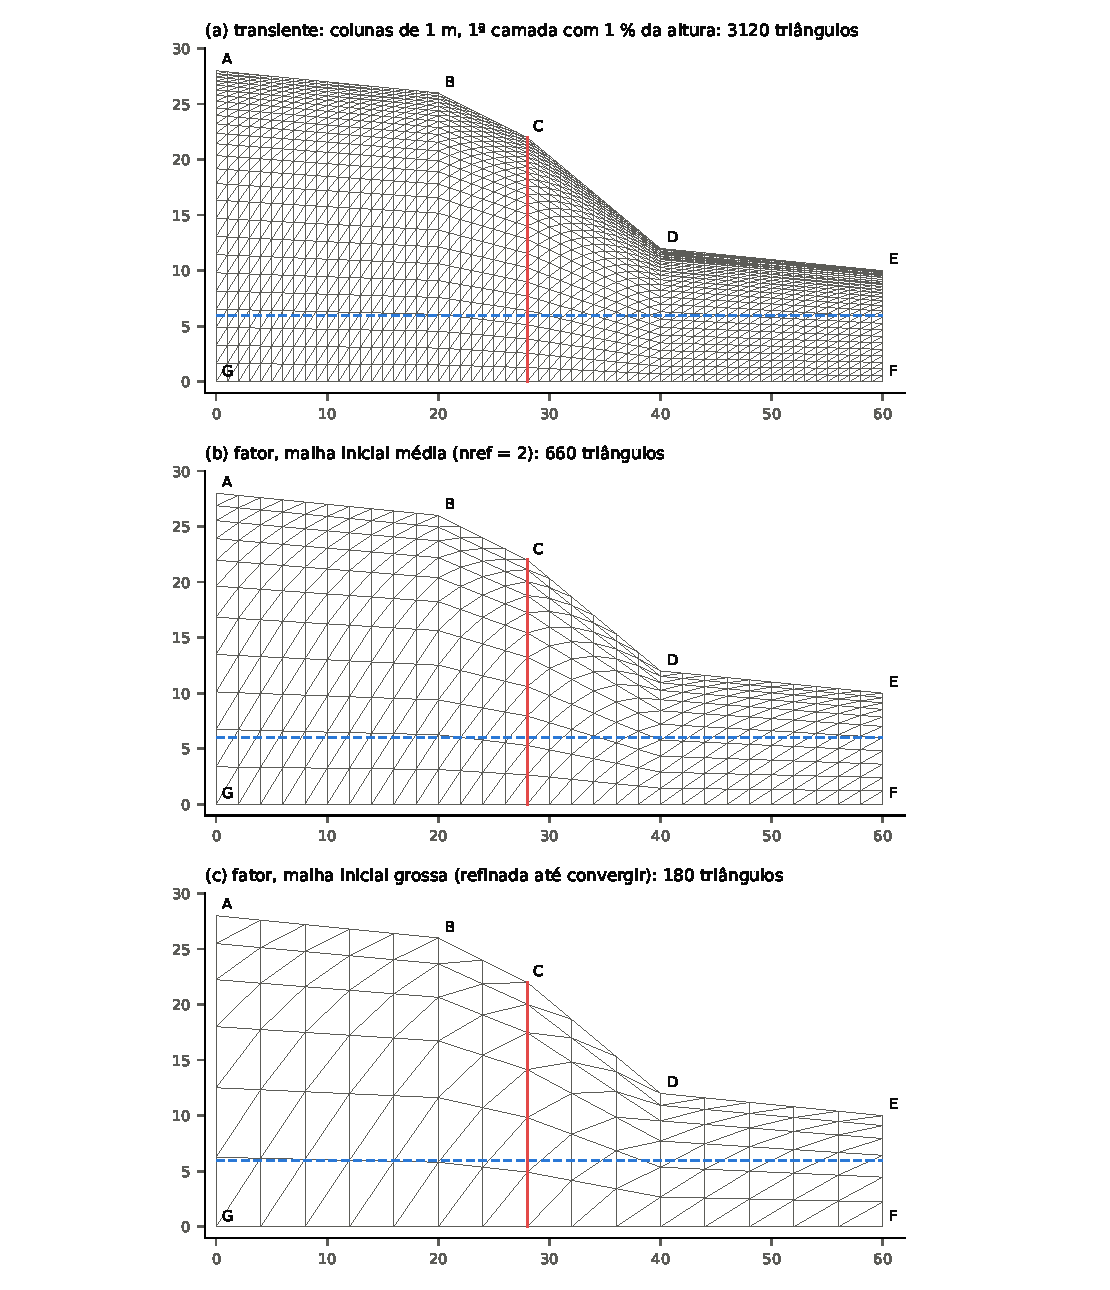
\includegraphics[width=0.85\textwidth]{figs/malhas.pdf}
\caption{As malhas (camadas que seguem a superfície). Tracejado azul: o nível d'água inicial; vermelho: a seção C--C'
($x = 28$~m).}\label{fig:malhas}
\end{figure}

\section{Fator de segurança inicial}
Com a malha grossa refinada até convergir, o FS inicial é 1,678; 1,605; 1,589; 1,578; 1,576 (4 refinamentos): o FS
convergido é \textbf{1,576} no silte (artigo 1,55, $+1{,}7\,\%$). Na areia, com a malha média e 2 níveis, 1,307
(artigo 1,22, $+7\,\%$). A diferença maior na areia é coerente com o fluxo associado: com $\phi' = 35^\circ$ o efeito da
dilatância no SRM é maior que com $30^\circ$.

\section{Dilatância}\label{sec:psi}
Com $\psi = \phi'$ o PV dá exatamente o FS do PV2 (Tab.~\ref{tab:psi}): a troca de material está certa. Com $\psi = 0$
o FS não é confiável: no silte ele sobe e desce com o refinamento, e na areia cai até 0,42 num talude que o artigo dá
como estável. É o comportamento conhecido do SRM com fluxo não associado: o arc-length perde a convergência (a matriz
tangente fica não simétrica e pode amolecer antes do colapso) e isso é tomado por ruptura. O teste com
$\psi = 10^{-6}$ graus separa um problema numérico do zero exato de um problema do não associado.
\afazer{o resultado de $\psi = 10^{-6}$}

\begin{table}[H]\centering\small
\caption{O FS inicial ($t = 0$) com o fluxo associado e com $\psi \approx 0$.}\label{tab:psi}
\begin{tabular}{ll|l|c}
\toprule
solo & material & FS em cada nível (malha média, 2 níveis) & Cho\\
\midrule
silte & PV2, $\psi = \phi'$ & 1{,}628; 1{,}588; 1{,}579 & 1,55\\
silte & PV, $\psi = \phi'$ & 1{,}628; 1{,}588; 1{,}579 & 1,55\\
silte & PV, $\psi = 0$ & 1{,}580; 1{,}401; 1{,}447 & 1,55\\
silte & PV, $\psi = 10^{-6}$ graus & (rodando) & 1,55\\
areia & PV2, $\psi = \phi'$ & 1{,}335; 1{,}314; 1{,}307 & 1,22\\
areia & PV, $\psi = \phi'$ & 1{,}335; 1{,}314; 1{,}307 & 1,22\\
areia & PV, $\psi = 0$ & 1{,}165; 0{,}810; 0{,}420 & 1,22\\
areia & PV, $\psi = 10^{-6}$ graus & (rodando) & 1,22\\
\bottomrule
\end{tabular}

\end{table}

\section{Silte: FS ao longo do tempo}

\begin{figure}[H]\centering
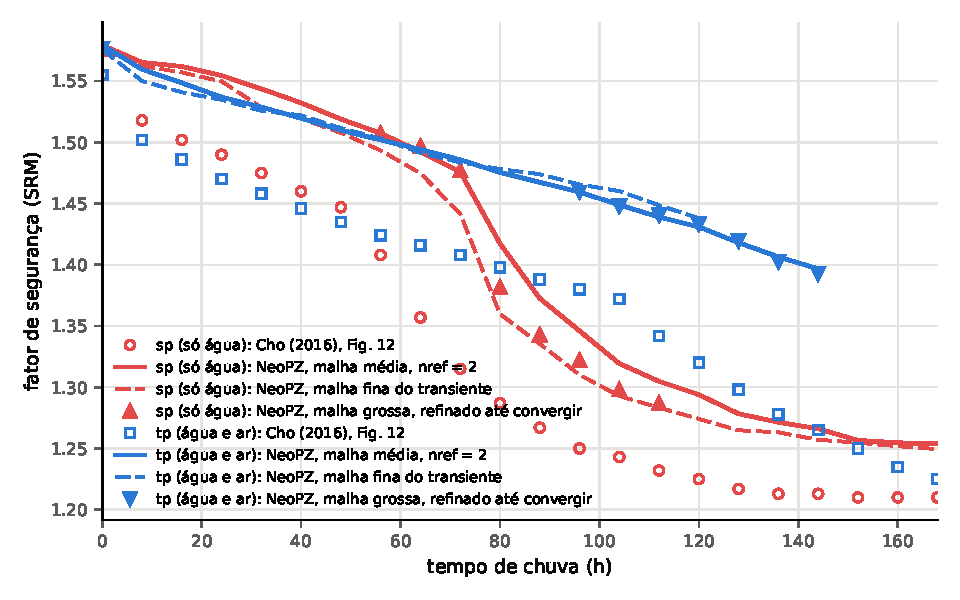
\includegraphics[width=0.9\textwidth]{figs/fs_silte.pdf}
\caption{Silte: o FS contra o tempo de chuva, NeoPZ contra a Fig.~12b de Cho (2016) (marcadores vazios, lidos a olho,
$\pm 0{,}01$). Linhas cheias: a malha do transiente atual, o FS na malha média com 2 níveis; triângulos: o FS na malha
grossa refinada até convergir; tracejadas: a malha fina do transiente (associado e $\psi \approx 0$), quando
existem.}\label{fig:fssilte}
\end{figure}

\begin{table}[H]\centering\small
\caption{Silte: o FS, NeoPZ (nref 2: malha média, 2 níveis; conv.: malha grossa refinada até convergir) e Cho (lido
da Fig.~12b); dif.: o melhor NeoPZ menos o Cho.}\label{tab:fssilte}
\begin{tabular}{r|ccccc|ccccc}
\toprule
 & \multicolumn{5}{c|}{sp (só água)} & \multicolumn{5}{c}{tp (água e ar)}\\
$t$ (h) & nref 2 & conv. & fina & Cho & dif. & nref 2 & conv. & fina & Cho & dif.\\
\midrule
0 & 1{,}579 & 1{,}576 & 1{,}576 & 1{,}55 & +0{,}02 & 1{,}579 & 1{,}576 & 1{,}576 & 1{,}55 & +0{,}02\\
8 & 1{,}565 & -- & 1{,}562 & 1{,}52 & +0{,}04 & 1{,}560 & -- & 1{,}550 & 1{,}50 & +0{,}05\\
16 & 1{,}562 & -- & 1{,}557 & 1{,}50 & +0{,}06 & 1{,}549 & -- & 1{,}541 & 1{,}49 & +0{,}05\\
24 & 1{,}555 & -- & 1{,}550 & 1{,}49 & +0{,}06 & 1{,}537 & -- & 1{,}535 & 1{,}47 & +0{,}06\\
32 & 1{,}544 & -- & 1{,}529 & 1{,}48 & +0{,}05 & 1{,}529 & -- & 1{,}526 & 1{,}46 & +0{,}07\\
40 & 1{,}532 & -- & 1{,}519 & 1{,}46 & +0{,}06 & 1{,}520 & -- & 1{,}522 & 1{,}45 & +0{,}08\\
48 & 1{,}519 & -- & 1{,}508 & 1{,}45 & +0{,}06 & 1{,}510 & -- & 1{,}512 & 1{,}44 & +0{,}08\\
56 & 1{,}507 & 1{,}508 & 1{,}493 & 1{,}41 & +0{,}09 & 1{,}502 & -- & 1{,}503 & 1{,}42 & +0{,}08\\
64 & 1{,}492 & 1{,}497 & 1{,}475 & 1{,}36 & +0{,}12 & 1{,}494 & -- & 1{,}491 & 1{,}42 & +0{,}08\\
72 & 1{,}476 & 1{,}477 & 1{,}442 & 1{,}31 & +0{,}13 & 1{,}486 & -- & 1{,}484 & 1{,}41 & +0{,}08\\
80 & 1{,}417 & 1{,}382 & 1{,}360 & 1{,}29 & +0{,}07 & 1{,}475 & -- & 1{,}478 & 1{,}40 & +0{,}08\\
88 & 1{,}373 & 1{,}343 & 1{,}336 & 1{,}27 & +0{,}07 & 1{,}467 & -- & 1{,}474 & 1{,}39 & +0{,}09\\
96 & 1{,}346 & 1{,}322 & 1{,}310 & 1{,}25 & +0{,}06 & 1{,}459 & 1{,}459 & 1{,}466 & 1{,}38 & +0{,}09\\
104 & 1{,}319 & 1{,}298 & 1{,}293 & 1{,}24 & +0{,}05 & 1{,}449 & 1{,}448 & 1{,}460 & 1{,}37 & +0{,}09\\
112 & 1{,}305 & 1{,}287 & 1{,}283 & 1{,}23 & +0{,}05 & 1{,}439 & 1{,}440 & 1{,}449 & 1{,}34 & +0{,}11\\
120 & 1{,}294 & -- & 1{,}274 & 1{,}23 & +0{,}05 & 1{,}431 & 1{,}433 & 1{,}438 & 1{,}32 & +0{,}12\\
128 & 1{,}278 & -- & 1{,}265 & 1{,}22 & +0{,}05 & 1{,}418 & 1{,}419 & -- & 1{,}30 & +0{,}12\\
136 & 1{,}271 & -- & 1{,}263 & 1{,}21 & +0{,}05 & 1{,}406 & 1{,}402 & -- & 1{,}28 & +0{,}12\\
144 & 1{,}266 & -- & 1{,}257 & 1{,}21 & +0{,}04 & 1{,}397 & 1{,}393 & -- & 1{,}26 & +0{,}13\\
152 & 1{,}257 & -- & 1{,}255 & 1{,}21 & +0{,}04 & -- & -- & -- & 1{,}25 & --\\
160 & 1{,}255 & -- & 1{,}252 & 1{,}21 & +0{,}04 & -- & -- & -- & 1{,}24 & --\\
168 & 1{,}254 & -- & 1{,}249 & 1{,}21 & +0{,}04 & -- & -- & -- & 1{,}23 & --\\
\bottomrule
\end{tabular}

\end{table}

O que se reproduz:
\begin{itemize}
  \item No início o tp cai mais rápido que o sp: com ar ativo, o ar comprimido sob a frente reduz a sucção antes.
  \item O sp tem uma queda forte, que no artigo vai de 56 a 96~h e aqui de 72 a 112~h: é a superfície de ruptura que sobe
    de profunda para rasa quando a frente avança (Seção~4.3 do artigo). Nesses instantes o refinamento demora mais a
    convergir (Tab.~\ref{tab:niveis}), porque a superfície rasa é estreita.
  \item No fim o tp fica acima do sp: o ar preso atrasa a frente.
\end{itemize}
O que não se reproduz: as nossas curvas vão atrasadas, porque a nossa frente de molhamento é mais lenta
(Seção~\ref{sec:frente}).

No fim (168~h) o sp chega a 1,254 (artigo 1,21) e o tp a 1,40 em 144~h (artigo 1,265). O refinamento até convergir
confirma os 2 níveis da malha média: as diferenças ficam abaixo de 0,005 nos instantes já calculados. O que falta é o
transiente.

\section{Silte: a frente de molhamento}\label{sec:frente}

\begin{figure}[H]\centering
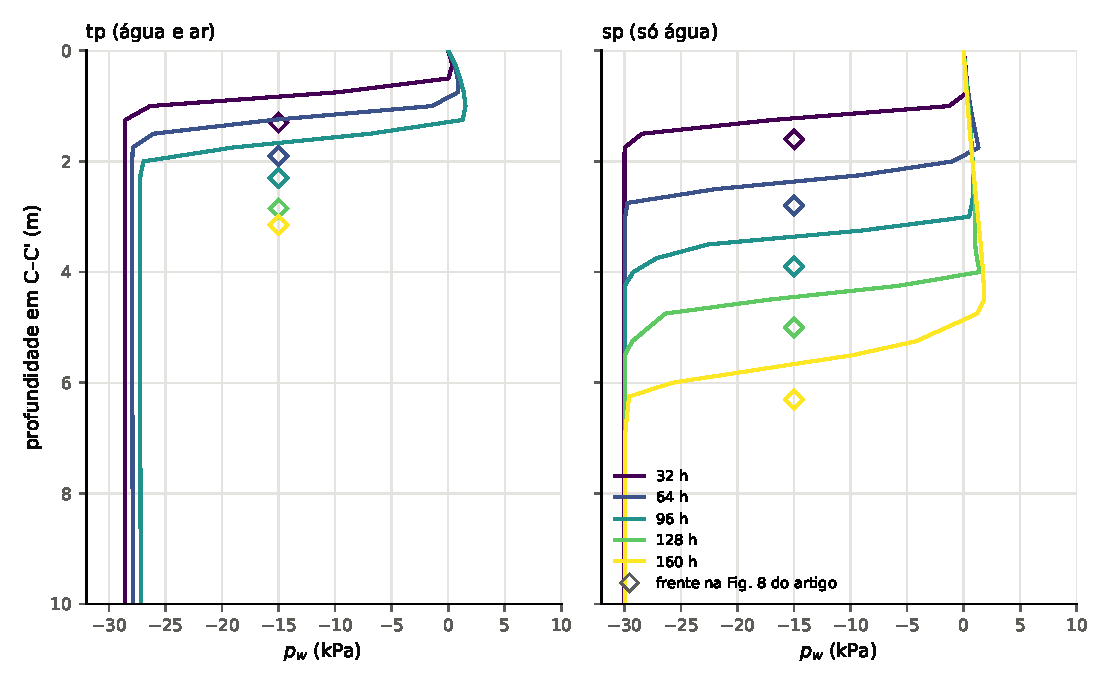
\includegraphics[width=0.85\textwidth]{figs/perfis_silte.pdf}
\caption{Silte: perfis de $p_w$ na seção C--C' (NeoPZ, malha do transiente atual) e o meio da frente na Fig.~8 do
artigo (losangos, $p_w = -15$~kPa, $\pm 0{,}2$~m).}\label{fig:perfis}
\end{figure}

\begin{table}[H]\centering\small
\caption{Silte: profundidade (m) do meio da frente ($p_w = -15$~kPa) em C--C', NeoPZ (malha atual) e Cho
(Fig.~8).}\label{tab:frente}
\begin{tabular}{r|cc|cc}
\toprule
 & \multicolumn{2}{c|}{sp} & \multicolumn{2}{c}{tp}\\
$t$ (h) & NeoPZ & Cho & NeoPZ & Cho\\
\midrule
32 & 1{,}06 & 1{,}60 & 0{,}82 & 1{,}30\\
64 & 2{,}00 & 2{,}80 & 1{,}22 & 1{,}90\\
96 & 3{,}08 & 3{,}90 & 1{,}61 & 2{,}30\\
128 & 4{,}11 & 5{,}00 & 1{,}99 & 2{,}85\\
160 & 5{,}33 & 6{,}30 & -- & 3{,}15\\
\bottomrule
\end{tabular}

\end{table}

\paragraph{Teste de malha do transiente.} O sp do silte em três malhas (Tab.~\ref{tab:malhat}): a frente desce mais
rápido quanto mais fina a malha, e ainda não convergiu; a 64~h, 1,5~m na grossa, 2,0~m na atual e 2,5~m na fina,
contra 2,8~m no artigo. A malha fina já está rodando com o FS (sp e tp, associado e $\psi \approx 0$). A causa é a malha em camadas por fração da altura: em C--C', com
22~m de solo, a primeira camada da malha atual tem 0,22~m, grossa para uma frente íngreme num solo que parte com
$S_w \approx 0{,}39$. A correção é usar camadas de espessura fixa (poucos centímetros) até a profundidade que a frente
alcança ($\approx 8$~m) e crescer só abaixo. \afazer{a malha nova e o silte refeito}

\begin{table}[H]\centering\small
\caption{Silte, sp: profundidade (m) do meio da frente em C--C' em três malhas do transiente.}\label{tab:malhat}
\begin{tabular}{lcc|cccc}
\toprule
malha & colunas & 1ª camada & \multicolumn{4}{c}{frente (m) a 16, 32, 48, 64 h}\\
\midrule
grossa & 2 m & 2\,\% & 0{,}50 & 0{,}69 & 1{,}09 & 1{,}46\\
atual & 1 m & 1\,\% & 0{,}57 & 1{,}06 & 1{,}53 & 2{,}00\\
fina & 0,5 m & 0,5\,\% & 0{,}69 & 1{,}22 & 1{,}78 & 2{,}36\\
\bottomrule
\end{tabular}

\end{table}

\section{Silte: os pontos de monitoramento}
H, I e J estão na vertical $x = 34$~m da face CD (posições lidas da Fig.~1, $\pm 0{,}2$~m): H $(34; 16{,}1)$,
I $(34; 15{,}1)$ e J $(34; 12{,}2)$, a $\approx 0{,}9$, 1,9 e 4,8~m abaixo da superfície. O driver grava $p_w$, $p_a$ e
a sucção neles de hora em hora (\texttt{*\_pontos.csv}).

\begin{figure}[H]\centering
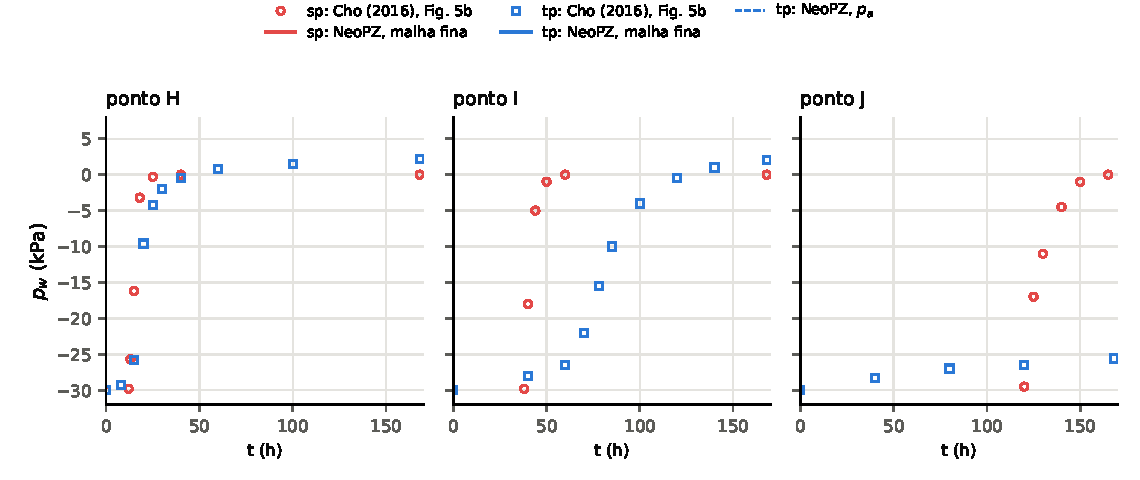
\includegraphics[width=\textwidth]{figs/pontos_silte.pdf}
\caption{Silte: $p_w$ nos pontos H, I e J, NeoPZ com a malha fina do transiente (linhas; tracejada: $p_a$ no tp)
contra a Fig.~5b de Cho (2016) (marcadores, lidos a olho, $\pm 1$~kPa e $\pm 3$~h).}\label{fig:pontos}
\end{figure}

\section{Areia}
O FS inicial converge (1,307), mas o transiente não passa de 0,02--0,15~h: o Newton diverge no início da chuva. A
$-30$~kPa a areia tem $S_w \approx 0{,}09$ e $k_r \approx 10^{-6}$, e a chuva de $3k_s$ chega a um solo que quase não
deixa a água entrar; refinar a malha perto da superfície fez parar ainda mais cedo. \afazer{passo inicial menor,
rampa na chuva, ou continuação na sucção inicial}

\begin{figure}[H]\centering
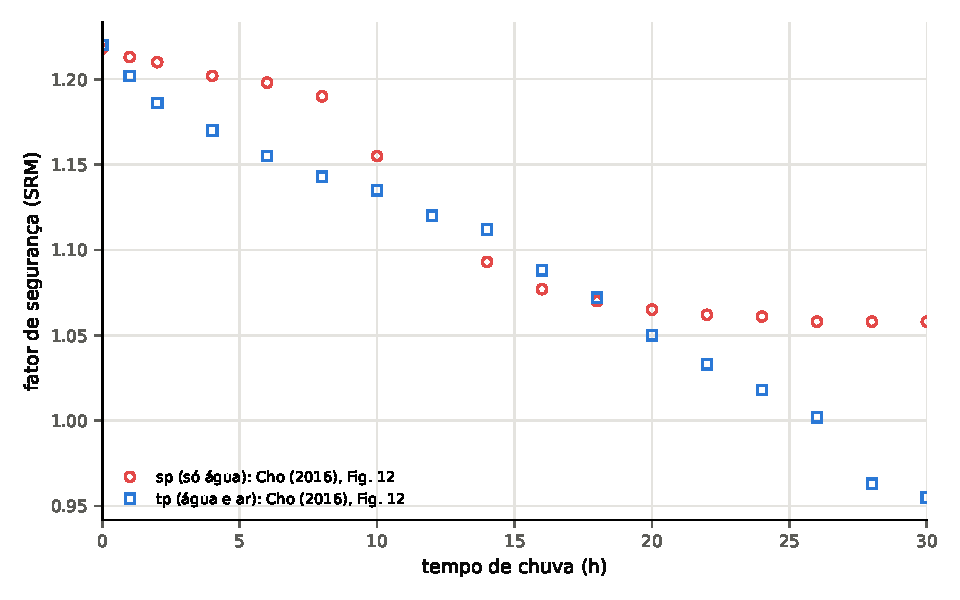
\includegraphics[width=0.75\textwidth]{figs/fs_areia.pdf}
\caption{Areia: a Fig.~12a de Cho (2016) (lida); o NeoPZ ainda só tem o FS inicial.}
\end{figure}

\section{Refinamento adaptativo do FS}
\begin{table}[H]\centering\scriptsize
\caption{Silte: o FS em cada nível do refinamento adaptativo.}\label{tab:niveis}
\begin{tabular}{llr|l}
\toprule
rodada & modelo & $t$ (h) & FS em cada nível (malha inicial, 1º refinamento, ...)\\
\midrule
média, nref 2 & sp & 0 & 1{,}628; 1{,}588; 1{,}579\\
média, nref 2 & sp & 8 & 1{,}612; 1{,}575; 1{,}565\\
média, nref 2 & sp & 16 & 1{,}606; 1{,}569; 1{,}562\\
média, nref 2 & sp & 24 & 1{,}601; 1{,}561; 1{,}555\\
média, nref 2 & sp & 32 & 1{,}589; 1{,}550; 1{,}544\\
média, nref 2 & sp & 40 & 1{,}569; 1{,}537; 1{,}532\\
média, nref 2 & sp & 48 & 1{,}555; 1{,}526; 1{,}519\\
média, nref 2 & sp & 56 & 1{,}543; 1{,}514; 1{,}507\\
média, nref 2 & sp & 64 & 1{,}528; 1{,}496; 1{,}492\\
média, nref 2 & sp & 72 & 1{,}505; 1{,}478; 1{,}476\\
média, nref 2 & sp & 80 & 1{,}472; 1{,}456; 1{,}417\\
média, nref 2 & sp & 88 & 1{,}445; 1{,}415; 1{,}373\\
média, nref 2 & sp & 96 & 1{,}423; 1{,}382; 1{,}346\\
média, nref 2 & sp & 104 & 1{,}398; 1{,}351; 1{,}319\\
média, nref 2 & sp & 112 & 1{,}377; 1{,}337; 1{,}305\\
média, nref 2 & sp & 120 & 1{,}364; 1{,}326; 1{,}294\\
média, nref 2 & sp & 128 & 1{,}342; 1{,}307; 1{,}278\\
média, nref 2 & sp & 136 & 1{,}331; 1{,}298; 1{,}271\\
média, nref 2 & sp & 144 & 1{,}321; 1{,}287; 1{,}266\\
média, nref 2 & sp & 152 & 1{,}308; 1{,}275; 1{,}257\\
média, nref 2 & sp & 160 & 1{,}302; 1{,}269; 1{,}255\\
média, nref 2 & sp & 168 & 1{,}297; 1{,}266; 1{,}254\\
média, nref 2 & tp & 0 & 1{,}628; 1{,}588; 1{,}579\\
média, nref 2 & tp & 8 & 1{,}606; 1{,}568; 1{,}560\\
média, nref 2 & tp & 16 & 1{,}595; 1{,}559; 1{,}549\\
média, nref 2 & tp & 24 & 1{,}584; 1{,}545; 1{,}537\\
média, nref 2 & tp & 32 & 1{,}574; 1{,}534; 1{,}529\\
média, nref 2 & tp & 40 & 1{,}559; 1{,}525; 1{,}520\\
média, nref 2 & tp & 48 & 1{,}555; 1{,}516; 1{,}510\\
média, nref 2 & tp & 56 & 1{,}544; 1{,}506; 1{,}502\\
média, nref 2 & tp & 64 & 1{,}533; 1{,}498; 1{,}494\\
média, nref 2 & tp & 72 & 1{,}522; 1{,}491; 1{,}486\\
média, nref 2 & tp & 80 & 1{,}510; 1{,}479; 1{,}475\\
média, nref 2 & tp & 88 & 1{,}500; 1{,}471; 1{,}467\\
média, nref 2 & tp & 96 & 1{,}489; 1{,}464; 1{,}459\\
média, nref 2 & tp & 104 & 1{,}482; 1{,}453; 1{,}449\\
média, nref 2 & tp & 112 & 1{,}477; 1{,}444; 1{,}439\\
média, nref 2 & tp & 120 & 1{,}471; 1{,}436; 1{,}431\\
média, nref 2 & tp & 128 & 1{,}459; 1{,}424; 1{,}418\\
média, nref 2 & tp & 136 & 1{,}446; 1{,}413; 1{,}406\\
média, nref 2 & tp & 144 & 1{,}434; 1{,}403; 1{,}397\\
grossa, até convergir & sp & 0 & 1{,}678; 1{,}605; 1{,}589; 1{,}578; 1{,}576\\
grossa, até convergir & sp & 56 & 1{,}595; 1{,}527; 1{,}517; 1{,}509; 1{,}508\\
grossa, até convergir & sp & 64 & 1{,}575; 1{,}520; 1{,}502; 1{,}497\\
grossa, até convergir & sp & 72 & 1{,}546; 1{,}503; 1{,}481; 1{,}477\\
grossa, até convergir & sp & 80 & 1{,}516; 1{,}484; 1{,}460; 1{,}420; 1{,}396; 1{,}386; 1{,}382\\
grossa, até convergir & sp & 88 & 1{,}500; 1{,}465; 1{,}417; 1{,}377; 1{,}353; 1{,}346; 1{,}343\\
grossa, até convergir & sp & 96 & 1{,}483; 1{,}447; 1{,}384; 1{,}350; 1{,}333; 1{,}324; 1{,}322\\
grossa, até convergir & sp & 104 & 1{,}473; 1{,}423; 1{,}354; 1{,}321; 1{,}308; 1{,}300; 1{,}298\\
grossa, até convergir & sp & 112 & 1{,}461; 1{,}399; 1{,}336; 1{,}308; 1{,}290; 1{,}287\\
grossa, até convergir & tp & 0 & 1{,}678; 1{,}605; 1{,}589; 1{,}578; 1{,}576\\
grossa, até convergir & tp & 96 & 1{,}555; 1{,}477; 1{,}467; 1{,}461; 1{,}459\\
grossa, até convergir & tp & 104 & 1{,}544; 1{,}469; 1{,}458; 1{,}450; 1{,}448\\
grossa, até convergir & tp & 112 & 1{,}533; 1{,}461; 1{,}449; 1{,}442; 1{,}440\\
grossa, até convergir & tp & 120 & 1{,}521; 1{,}454; 1{,}441; 1{,}435; 1{,}433\\
grossa, até convergir & tp & 128 & 1{,}504; 1{,}442; 1{,}427; 1{,}420; 1{,}419\\
grossa, até convergir & tp & 136 & 1{,}486; 1{,}430; 1{,}417; 1{,}404; 1{,}402\\
grossa, até convergir & tp & 144 & 1{,}469; 1{,}420; 1{,}405; 1{,}395; 1{,}393\\
\bottomrule
\end{tabular}

\end{table}

\section{Próximos passos}
\begin{enumerate}
  \item A malha do transiente com camadas de espessura fixa perto da superfície, até a frente convergir; refazer o
    silte (sp e tp) e comparar de novo com as Figs.~8 e 12b.
  \item A areia: fazer o transiente passar do início da chuva.
  \item A sucção e $p_a$ nos pontos (Fig.~6) e os perfis de $p_a$ (Fig.~9).
\end{enumerate}

\end{document}
